\documentclass{article}
\usepackage[T1]{fontenc}
\usepackage{lmodern}
\usepackage{graphicx}
\usepackage{amsmath,amssymb}
\usepackage[a4paper,margin=2cm]{geometry}
\usepackage[absolute,overlay]{textpos}
\setlength{\TPHorizModule}{1mm}
\setlength{\TPVertModule}{1mm}
\usepackage[indonesian]{babel}
\usepackage{hyperref}
\setlength{\emergencystretch}{2em}
% unit: Halaman 14

\begin{document}

% === Halaman 14 (python/native) ===

14

Hitung frekuensi kemunculan huruf di dalam cipherteks tersebut sbb:

𝐶𝐼=

෌𝑖=1

21 𝑓𝑖𝑓𝑖−1

𝑁𝑁−1

 = 

916

120(119) = 0,0641 

Jumlah total huruf, N = 120

Nilai CI sangat dekat dengan 0,065 (teks bahasa Inggris), jauh dari 0,038 (teks acak/polyalphabetic 

cipher), maka kemungkinan besar ini adalah cipherteks dari monoalphabetic cipher

% deskripsi: gambar native xref 77
\noindent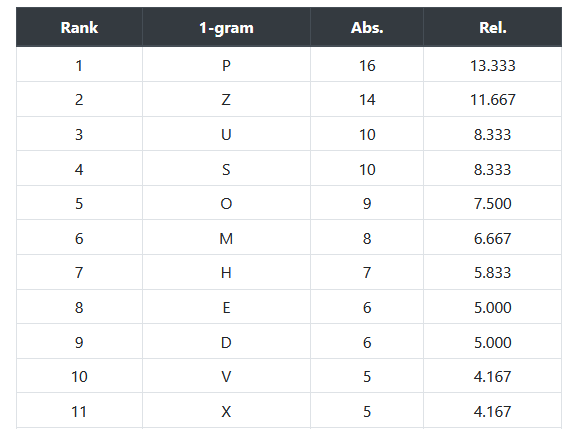
\includegraphics[width=0.85\textwidth]{../../images/python/page_014_img_01.png}

% deskripsi: gambar native xref 78
\noindent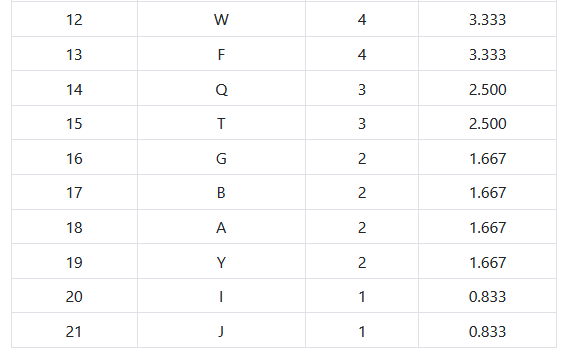
\includegraphics[width=0.85\textwidth]{../../images/python/page_014_img_02.png}

% deskripsi: gambar native xref 79
\noindent
\includegraphics[width=0.85\textwidth]{../../images/python/page_014_img_03.png}

\end{document}
